% !TeX root = hw_1-koncni_avtomati.tex
\documentclass{article}

\usepackage{forest}
\usepackage{graphicx}
\usepackage{tikz}
\usepackage{tikz-qtree}
\usepackage{parskip}
\usetikzlibrary {arrows.meta,automata,positioning}
\title{Algoritmi v bioinformatiki - 1. Domača naloga}
\author{Jan Panjan}
\date{\today}

\begin{document}

\tikzset{
	node distance=2.6cm, % specifies the minimum distance between two nodes. Change if necessary.
	every state/.style={thick, fill=gray!10}, % sets the properties for each ’state’ node
	->, % makes the edges directed
	>={Stealth} % make arrow heads bold
}

\maketitle
\newpage

\begin{enumerate}
	\item \textit{Konstruirajte deterministični končni avtomat, ki v mRNK materialu prepozna
		zaključne kodone.}
		\begin{enumerate}
			\item Grafično:

				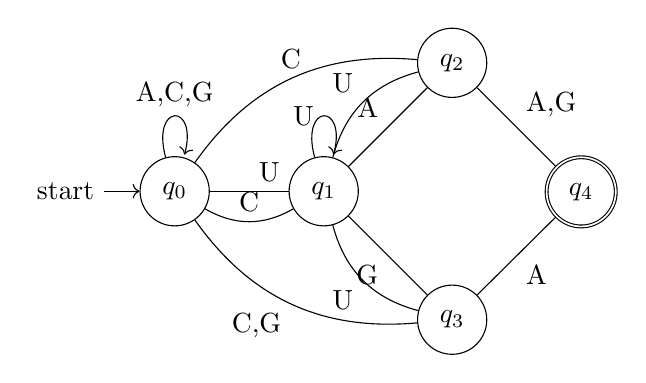
\begin{tikzpicture}
					\node[state, initial]   (q0)                     {$q_0$};
					\node[state] 			(q1) [right=of q0]       {$q_1$};
					\node[state] 	        (q2) [above right=of q1] {$q_2$};
					\node[state] 		    (q3) [below right=of q1] {$q_3$};
					\node[state, accepting] (q4) [below right=of q2] {$q_4$};

					\draw (q0) edge[loop above] node{A,C,G} (q0)
						(q0) edge[above right] node{U} (q1)

						(q1) edge[above, bend left] node{C} (q0)
						(q1) edge[above left] node{A} (q2)
						(q1) edge[below left] node{G} (q3)
						(q1) edge[loop above, left] node{U} (q1)

						(q2) edge[above left, bend right] node{U} (q1)
						(q2) edge[above right] node{A,G} (q4)
						(q2) edge[above, bend right] node{C} (q0)

						(q3) edge[below left, bend left] node{U} (q1)
						(q3) edge[bend left, below left] node{C,G} (q0)
						(q3) edge[below right] node{A} (q4);
				\end{tikzpicture}

			\item S formalnim opisom peterike $\left[ \Sigma, Q, q_0, F, \delta \right]$:

				\begin{itemize}
					\item $\Sigma = \{ A, U, C, G \}$
					\item $Q = \{ q_1, q_2, q_3, q_4 \}$
					\item $q_0 = q_0$
					\item $F = \{ q_4 \}$
					\item stanja so pisana samo s številko in pot ki pripelje do
						končnega stanja je označena z rdečo barvo, da je bolj
						berljivo.

						\begin{tabular}{|c||c|c|c|c|}
							\hline
							$\delta$ & A & U & C & G \\
							\hline \hline
							0 & 0 & \textcolor{red}{1} & 0 & 0 \\
							\hline
							1 & \textcolor{red}{2} & 1 & 0 & \textcolor{red}{3} \\
							\hline
							2 & \textcolor{red}{4} & 1 & 0 & \textcolor{red}{4} \\
							\hline
							3 & \textcolor{red}{4} & 1 & 0 & 0 \\
							\hline
							4 & / & / & / & / \\
							\hline
						\end{tabular}
				\end{itemize}
		\end{enumerate}

		\newpage

	\item \textit{Kako se rešitev 1. naloge spremeni, če želimo s pomočjo končnega
			avtomata poiskati vse pojavitve zaključnih kodonov? Zapišite algoritem
			in ponazorite njegovo delovanje na delu mRNK AUAUAAUGCUUGA. Koliko
		zaključnih kodonov vsebuje dani mRNK?}

		Njegovo končno stanje se spremeni, tako da ponovno začne iskati vzorec, ko
		pride enkrat do
		končnega stanja. To je vidno grafično kot povezava od $q_4$ do $q_0$ in
		spremenjene vrednosti v zadnji vrstici $\delta-$tabele.

		\begin{enumerate}
			\item Grafično:

				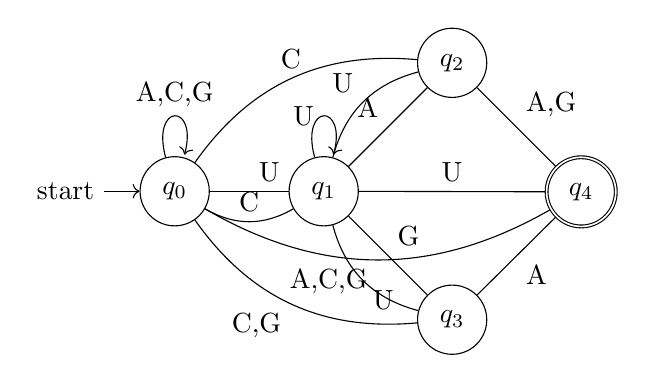
\begin{tikzpicture}
					\node[state, initial]   (q0)                     {$q_0$};
					\node[state] 			(q1) [right=of q0]       {$q_1$};
					\node[state] 	        (q2) [above right=of q1] {$q_2$};
					\node[state] 		    (q3) [below right=of q1] {$q_3$};
					\node[state, accepting] (q4) [below right=of q2] {$q_4$};

					\draw (q0) edge[loop above] node{A,C,G} (q0)
						(q0) edge[above right] node{U} (q1)

						(q1) edge[above, bend left] node{C} (q0)
						(q1) edge[above left] node{A} (q2)
						(q1) edge[above right] node{G} (q3)
						(q1) edge[loop above, left] node{U} (q1)

						(q2) edge[above left, bend right] node{U} (q1)
						(q2) edge[above right] node{A,G} (q4)
						(q2) edge[above, bend right] node{C} (q0)

						(q3) edge[below right, bend left] node{U} (q1)
						(q3) edge[bend left, below left] node{C,G} (q0)
						(q3) edge[below right] node{A} (q4)

						(q4) edge[above] node{U} (q1)
						(q4) edge[bend left, below left] node{A,C,G} (q0);
				\end{tikzpicture}

			\item S formalnim opisom peterike $\left[ \Sigma, Q, q_0, F, \delta \right]$:

				\begin{itemize}
					\item $\Sigma = \{ A, U, C, G \}$
					\item $Q = \{ q_1, q_2, q_3, q_4 \}$
					\item $q_0 = q_0$
					\item $F = \{ q_4 \}$
					\item \begin{tabular}{|c||c|c|c|c|}
							\hline
							$\delta$ & A & U & C & G \\
							\hline \hline
							0 & 0 & \textcolor{red}{1} & 0 & 0 \\
							\hline
							1 & \textcolor{red}{2} & 1 & 0 & \textcolor{red}{3} \\
							\hline
							2 & \textcolor{red}{4} & 1 & 0 & \textcolor{red}{4} \\
							\hline
							3 & \textcolor{red}{4} & 1 & 0 & 0 \\
							\hline
							4 & 0 & 1 & 0 & 0 \\
							\hline
						\end{tabular}
				\end{itemize}
		\end{enumerate}

		\textbf{Algoritem za iskanje STOP kodonov v mRNA vzorcu:} algoritem za izgradnjo
		$\delta-$tabele smo podali na vajah in ga ne bom ponovno napisal.
		Predpostavljam torej, da je tabela za naš končni avtomat že izgrajena.
		Iskanje vzorca v besedilu AUAUAAUGCUUGA poteka tako:

		kaj je mišljeno kot algoritem tu..? (poglej zapiske od vaj/predavanj, mislim da je podano)

		Dani vzorec mRNA vsebuje dva stop kodona: AUA\textcolor{red}{UAA}UGCU\textcolor{red}{UGA}

	\item \textit{Konstruirajte determinističen končni avtomat za naslednji
		nedeterminističen končni avtomat.}

		Deterministični končni avtomat iz nedeterminističnega izgradimo s pomočjo
		$\delta-$tabele tako da zapišemo vse neprazne podmnožice stanj. Za stanje
		npr. $1,2$ naredimo unijo sledečih stanj za $a$ in $b$, t.j $1,2,3$ in $2$., t.j $1,2,3$ in
		$2$. Da se izognemo pisanju nepotrebnih stanj, naredimo tabelo samo za dosegljiva
		stanja.

		\textbf{Nedeterminističen končni avtomat:}

		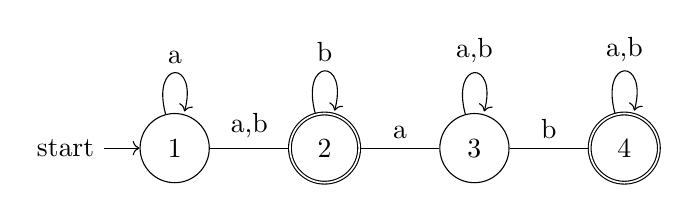
\begin{tikzpicture}
			\node[state, initial]   (q1)               {$1$};
			\node[state, accepting]	(q2) [right=of q1] {$2$};
			\node[state] 	        (q3) [right=of q2] {$3$};
			\node[state, accepting] (q4) [right=of q3] {$4$};

			\draw (q1) edge[loop above] node{a} (q1)
				(q1) edge[above] node{a,b} (q2)
				(q2) edge[loop above] node{b} (q2)
				(q2) edge[above] node{a} (q3)
				(q3) edge[loop above] node{a,b} (q3)
				(q3) edge[above] node{b} (q4)
				(q4) edge[loop above] node{a,b} (q4);
		\end{tikzpicture}

		\textbf{$\delta-$tabela:}

		\begin{tabular}{|c||c|c|}
			\hline
			$\delta$ & a & b \\
			\hline\hline
			1 & 1,2 & 2 \\
			\hline
			2 & 3 & 2 \\
			\hline
			3 & 3 & 3,4 \\
			\hline
			4 & 4 & 4 \\
			\hline
			1,2 & 1,2,3 & 2 \\
			\hline
			3,4 & 3,4 & 3,4 \\
			\hline
			1,2,3 & 1,2,3 & 2,3,4 \\
			\hline
			2,3,4 & 3,4 & 2,3,4 \\
			\hline
		\end{tabular}

		Končna stanja sta $2$ in $4$, zato bo imel novi končni avtomat za končna
		stanja vsa stanja, ki vsebujejo tako $2$ ali $4$.

		Zgodi se, da stanje $4$ odpade, saj nobeno stanje ne vodi vanj.

		\textbf{Determinističen končni avtomat:}

		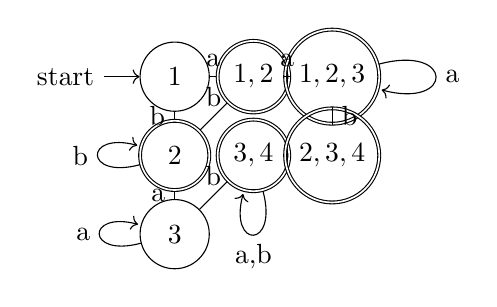
\begin{tikzpicture}
			\node[state, initial] (1) {$1$};
			\node[state, accepting] (2) [below of=1] {$2$};
			\node[state] (3) [below of=2] {$3$};
			\node[state, accepting] (12) [right of=1] {$1,2$};
			\node[state, accepting] (123) [right of=12] {$1,2,3$};
			\node[state, accepting] (34) [below of=12] {$3,4$};
			\node[state, accepting] (234) [below of=123] {$2,3,4$};

			\draw (1) edge[left] node{b} (2)
				(1) edge[above] node{a} (12)
				(12) edge[above] node{b} (2)
				(12) edge[above] node{a} (123)
				(123) edge[loop right] node{a} (123)
				(123) edge[right] node{b} (234)
				(2) edge[loop left] node{b} (2)
				(2) edge[left] node{a} (3)
				(3) edge[loop left] node{a} (3)
				(3) edge[above] node{b} (34)
				(34) edge[loop below] node{a,b} (34);
		\end{tikzpicture}

	\item \textit{Poleg postopka z uporabo končnih avtomatov, poznamo tudi druge načine, kako
			odgovoriti na vprašanje "Kje in kolikokrat se vzorec p pojavi v besedilu t"? Naj bo naše
		besedilo $t$ = ACCACCGACGCCCGA.}

		\begin{enumerate}
			\item \textit{Za vzorec $p$ = CCGA, ponazorite delovanje algoritma KMP tako, da poiščete
					vzorec $p$ v besedilu $t$ in opišite, kako nam pri tem pomaga funkcija $\pi$.
				Kolikokrat in kje se vzorec $p$ pojavi v besedilu $t$?}

				KMP ali Knuth-Moriss-Prath-ov algoritem deluje na principu najdaljše predpone vzorca,
				ki je tudi pripona v dotedaj preiskanem besedilu. Z uporabo $\pi-$funkcije se
				algoritem izogne nepotrebnim primerjavam znakov v besedilu, za katere že vemo, da
				se ujemajo na začetku vzorca.

				S funkcijo $\pi$ najdemo najdaljšo predpono vzorca, ki je tudi njegova najdaljša
				pripona. Za naš vzorec izgleda tako:

				\begin{center}
					\begin{tabular}{c|c c c c}
						$p$ & C & C & G & A \\
						\hline
						$\pi(p)$ & 0 & 1 & 0 & 0 \\
					\end{tabular}
				\end{center}

				Psevdokoda za algoritem KMP izgleda tako:

				\begin{verbatim}
					def KMP(t, p):
						n = |t|
						m = |p|
						pi = Construct(p) // izgradi zgornji pi-seznam
						r = []            // seznam ki hrani začetne indekse
											 //         kjer se pojavi ujemanje
						q = 0

						for i = 1 to n - 1:
							while q > 0 and p[q + 1] is not t[i]:
									q = pi

							   if p[q + 1] == t[i]:
									q += 1

								  if q == m:
									   r = r.add(i - q + 1)

						   return r
				\end{verbatim}

				Potek algoritma je opisan z naslednjo tabelo:

				\begin{tabular}{|c|c|c|c|c|c|}
					\hline
					$q$ & $i$ & $p[q+1]$ & $t[i]$ & match & action \\
					\hline\hline
					0 & 1 & C & A & No & incr i \\
					\hline
					0 & 2 & C & C & Yes & incr q,i \\
					\hline
					1 & 3 & C & C & Yes & incr q,i \\
					\hline
					2 & 4 & G & A & No & $q=\pi[2]=1$ \\
					\hline
					1 & 4 & C & A & No & $q=\pi[1]=0$ \\
					\hline
					0 & 4 & C & A & No & incr i \\
					\hline
					0 & 5 & C & C & Yes & incr q,i \\
					\hline
					1 & 6 & C & C & Yes & incr q,i \\
					\hline
					2 & 7 & G & G & Yes & incr q,i \\
					\hline
					3 & 8 & A & A & Yes & incr q,i \\
					\hline
					4 & 9 & $\epsilon$ & C & No & $r.add(i-q+1)$, $q=\pi[4]$ \\
					\hline
					0 & 9 & C & C & Yes & incr q,i \\
					\hline
					1 & 10 & C & G & No & $q=\pi[1]$ \\
					\hline
					0 & 10 & C & G & No & incr i \\
					\hline
					0 & 11 & C & C & Yes & incr q,i \\
					\hline
					1 & 12 & C & C & Yes & incr q,i \\
					\hline
					2 & 13 & G & C & No & $q=\pi[2]$ \\
					\hline
					1 & 13 & C & C & Yes & incr q,i \\
					\hline
					2 & 14 & G & G & Yes & incr q,i \\
					\hline
					3 & 15 & A & A & Yes & incr q,i \\
					\hline
					4 & 16 & $\epsilon$ & $\epsilon$ & - & $r.add(i-q+1)$, $i=m:STOP$ \\
					\hline
				\end{tabular}

				Vzorec se pojavi dvakrat v našem besedilu. Algoritem najde ujemanja na indeksih
				5 in 12.

			\item \textit{Zgradite priponsko drevo za besedilo $t$. Opišite, kako s pomočjo
					priponskega drevesa učinkovito odgovorimo na vprašanje "Kje in kolikokrat se v
				besedilu $t$ pojavi aminokislina prolin?"}

				Priponsko drevo izgradimo tako, da najprej najdemo vse pripone našega besedila $t$,
				nato pa jih (po abecednem vrstnem redu) dodajamo v drevo z začetkom v korenu.
				Pripone, ki imajo enako pripono bodo sledile istemu poddrevesu, a ga bodo nato
				razcepile na več podvej. V listih drevesa hranimo začetni indeks pripone.

				Vse pripone našega besedila:

				1. ACCACCGACGCCCGA\$

				2. CCACCGACGCCCGA\$

				3. CACCGACGCCCGA\$

				4. ACCGACGCCCGA\$

				5. CCGACGCCCGA\$

				6. CGACGCCCGA\$

				7. GACGCCCGA\$

				8. ACGCCCGA\$

				9. CGCCCGA\$

				10. GCCCGA\$

				11. CCCGA\$

				12. CCGA\$

				13. CGA\$

				14. GA\$

				15. A\$

				16. \$

				Indeksi urejeni po abedecnem vrstnem redu:

				\begin{center}
					16, 15, 1, 4, 8, 3, 2, 11, 12, 5, 13, 6, 9, 14, 7, 10
				\end{center}

				Iz tega zdaj izgradimo priponsko drevo. Razdelil sem ga na 3 slike. Vsaka slika
				vsebuje poddrevesa, ki se začnejo s svojo črko (torej A, C in G).

				(mislim, da je boljše da samo prilepiš slike na roke narisane)

				\begin{tikzpicture}[
					every tree node/.style={draw,circle,inner sep=2pt,minimum size=6pt,font=\scriptsize},
					blank/.style={draw=none},
					edge from parent/.style={draw,->},
					level distance=1cm,
					sibling distance=0.4cm
					]
					\Tree [.A
					[.C
					[.C
					[.A
					[.C
					[.C
					[.G
					[.A
					[.C
					[.G
					[.C
					[.C
					[.C
					[.G
					[.A
					[.\$ \edge node[auto,swap,font=\tiny] {1, 4, 8, 15}; ]
					]
					]
					[.G
					[.A
					[.\$ \edge node[auto,swap,font=\tiny] {11}; ]
					]
					]
					]
					[.G
					[.A
					[.\$ \edge node[auto,swap,font=\tiny] {10}; ]
					]
					]
					]
					[.C
					[.C
					[.C
					[.G
					[.A
					[.\$ \edge node[auto,swap,font=\tiny] {12}; ]
					]
					]
					[.G
					[.A
					[.\$ \edge node[auto,swap,font=\tiny] {13}; ]
					]
					]
					]
					[.G
					[.A
					[.\$ \edge node[auto,swap,font=\tiny] {14}; ]
					]
					]
					]
					]
					]
					]
					]
					]
					]
					]
					]
					[.G
					[.A
					[.C
					[.G
					[.C
					[.C
					[.C
					[.G
					[.A
					[.\$ \edge node[auto,swap,font=\tiny] {2}; ]
					]
					]
					]
					]
					]
					]
					]
					]
					]
					]
					]
					[.C
					[.C
					[.G
					[.A
					[.C
					[.G
					[.C
					[.C
					[.C
					[.G
					[.A
					[.\$ \edge node[auto,swap,font=\tiny] {3}; ]
					]
					]
					]
					]
					]
					]
					]
					]
					]
					]
					]
					]
					[.\$ \edge node[auto,swap,font=\tiny] {16}; ]
					]
				\end{tikzpicture}

				\begin{tikzpicture}[
					every tree node/.style={draw,circle,inner sep=2pt,minimum size=6pt,font=\scriptsize},
					blank/.style={draw=none},
					edge from parent/.style={draw,->},
					level distance=1cm,
					sibling distance=0.4cm
					]
					\Tree [.C
					[.C
					[.A
					[.C
					[.C
					[.G
					[.A
					[.C
					[.G
					[.C
					[.C
					[.C
					[.G
					[.A
					[.\$ \edge node[auto,swap,font=\tiny] {5}; ]
					]
					[.G
					[.A
					[.\$ \edge node[auto,swap,font=\tiny] {12}; ]
					]
					]
					]
					[.G
					[.A
					[.\$ \edge node[auto,swap,font=\tiny] {11}; ]
					]
					]
					]
					[.G
					[.A
					[.\$ \edge node[auto,swap,font=\tiny] {10}; ]
					]
					]
					]
					[.C
					[.C
					[.C
					[.G
					[.A
					[.\$ \edge node[auto,swap,font=\tiny] {13}; ]
					]
					]
					[.G
					[.A
					[.\$ \edge node[auto,swap,font=\tiny] {14}; ]
					]
					]
					]
					[.G
					[.A
					[.\$ \edge node[auto,swap,font=\tiny] {15}; ]
					]
					]
					]
					]
					]
					]
					]
					]
					]
					]
					]
					]
					]
					[.G
					[.A
					[.C
					[.G
					[.C
					[.C
					[.C
					[.G
					[.A
					[.\$ \edge node[auto,swap,font=\tiny] {6}; ]
					]
					]
					]
					]
					]
					]
					]
					]
					]
					]
					]
				\end{tikzpicture}

				\begin{tikzpicture}[
					every tree node/.style={draw,circle,inner sep=2pt,minimum size=6pt,font=\scriptsize},
					blank/.style={draw=none},
					edge from parent/.style={draw,->},
					level distance=1cm,
					sibling distance=0.4cm
					]
					\Tree [.G
					[.A
					[.C
					[.G
					[.C
					[.C
					[.C
					[.G
					[.A
					[.\$ \edge node[auto,swap,font=\tiny] {7}; ]
					]
					]
					]
					]
					]
					]
					]
					]
					]
				\end{tikzpicture}

				\end{document}

		\end{enumerate}

\end{enumerate}

\end{document}
